\documentclass[a4paper, 10pt]{article}
\usepackage{helvet}
\renewcommand{\familydefault}{\sfdefault}
\usepackage{pgf}
\usepackage{eurosym}
\usepackage{graphicx}
\usepackage{wasysym}
\usepackage{hyperref}
\usepackage{listings}
\usepackage{pxfonts}
\usepackage{verbatim}
\usepackage{color}
\usepackage{xcolor}
\usepackage{wrapfig}
\usepackage{enumitem}
\usepackage{booktabs}
\usepackage{gensymb}
\usepackage{tabularx}
\usepackage{currfile}

\hypersetup{
    bookmarks=true,         % show bookmarks bar?
    unicode=true,          % non-Latin characters in Acrobat’s bookmarks
    pdftoolbar=true,        % show Acrobat’s toolbar?
    pdfmenubar=true,        % show Acrobat’s menu?
    pdffitwindow=true,     % window fit to page when opened
    pdftitle={Assessments},    % title
    pdfauthor={Paul Vesey},     % author
    pdfsubject={Building Information Modelling },   % subject of the document
    pdfcreator={},   % creator of the document
    pdfproducer={xelatex}, % producer of the document
    pdfkeywords={'Graphics' }, % list of keywords
    pdfnewwindow=true,      % links in new PDF window
    colorlinks=true,       % false: boxed links; true: colored links
    linkcolor=violet,          % color of internal links (change box color with linkbordercolor)
    citecolor=magenta,        % color of links to bibliography
    filecolor=red,      % color of file links
    urlcolor=blue           % color of external links
}

\setlength\parindent{0pt}
\begin{document}

\lstset{language=HTML,
				basicstyle=\small,
				breaklines=true,
        numbers=left,
        numberstyle=\tiny,
        showstringspaces=false,
        aboveskip=-20pt,
        frame=leftline
        }


\begin{figure}
	\centering
	\includegraphics[width=0.5\linewidth]{./img/TUSlogo}
\end{figure}


\begin{tabularx}{\textwidth}{ |l|X| }
	\hline
	
	\textbf{Subject:} & Health \& Safety IT\\
	\textbf{Course:} & BSc in Construction Health \& Safety\\
	\textbf{Session:} & Autumn 2021\\
	\textbf{Lecturer:} & Paul Vesey \footnotesize{BEng, MIE, HDip}\\
	\textbf{Filename:} & \currfilebase\\
	\hline
\end{tabularx}

	
\part*{Assignment 1 (25\%) - Microsoft Forms}

\begin{tabularx}{\textwidth}{ |X|X| }
	\hline
	\textbf{Issue Date:} & As stated on Moodle \\
	\hline 
	\textbf{Submission Date:}  & As stated on Moodle  \\
	\hline
\end{tabularx}


\section*{Assignment Outline}


In this assignment you will create an on-line survey to capture the prestart checks undertaken by a site dumper operator.  The platform for the on-line survey is to be Microsoft Forms, which is available through your Office 365 Student Subscription.


\section*{Background Information}

The HSA has a published document for Site Dumper Prestart checks.  This document is available in the assignment pack, and is available for download \href{https://www.hsa.ie/eng/Publications_and_Forms/Publications/Construction/Site_Dumper_and_360_Excavator_Pre-start_Checks.html}{here}.  An image is also shown in Fig \ref{fig:DumperPrestartChecks}

\begin{figure}
	\centering
	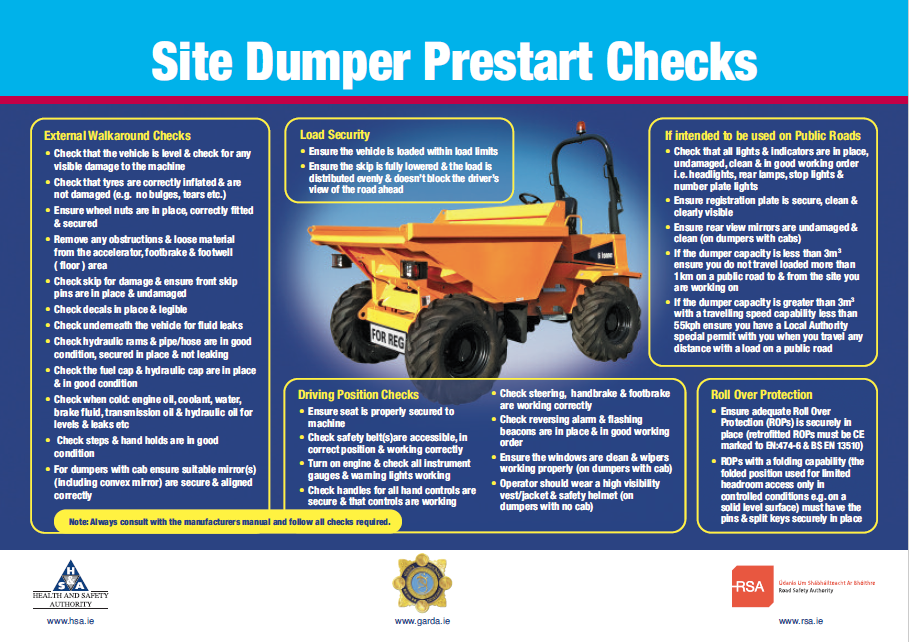
\includegraphics[width=1.0\linewidth]{img/DumperPrestart.png}
	\caption{Dumper Prestart Checks}
	\label{fig:DumperPrestartChecks}
\end{figure}

\section*{Usability}

Your final survey is intended to be deployed on site, for usage checks by drivers.  As such you should consider the following in the design and implementation of your survey:
\begin{itemize}
	\item Questions should be short and easy to read
	\item Responses should be clear and unambiguous
	\item Where failures are detected by the operator, additional information should be captured
\end{itemize}

\newpage
\section*{Functionality}

The following functionality must be included in your deployment:
\begin{itemize}
	\item Driver Name and Employee Number
	\item Dumper Registration
	\item All items as per the HSA document
	\item Appropriate Branching to capture comments on failed checks
	\item A branch specifically implemented for 'Use on Public Roads'
	\item A specific multi line input field for group testing feedback.
\end{itemize}

\section*{Testing}
Testing of your deployment will be done in two stages
\begin{enumerate}
	\item Author Testing - You should test your deployment rigorously before proceeding to the next stage
	\item Group Testing - Your Deployment will be tested by all other members of the class, and you will be expected to test all other deployments.
\end{enumerate}


\newpage
\section*{Group Testing Feedback}
Group testing will be implemented to improve your deployment prior to final submission. All feedback is to be:
\begin{itemize}
	\item Specific, meaningful \& constructive
	\item Impersonal
	\item Process Orientated
\end{itemize}

\section*{Submission}
This is a relatively complex submission, that will comprise many parts.  The parts are as follows:
\begin{enumerate}
	\item Link to Microsoft Form (with a .txt file)
	\item Screen-shots of the form before group testing, numbered appropriately
	\item Screen-shots of the form after group testing, numbered appropriately
	\item Excel file containing all responses, including comments from group testing
\end{enumerate}

All parts are to be compressed into a single zip folder compelete with logical sectioning.  The link to the form URL can be included in a simple text file in the submission.


\end{document}